% Two charts glued over [0,2] with a SMOOTH nonlinear transition phi_2,
% flat to infinite order at the overlap edge (bump x + exp(-1/(x-1))).
% Source: book/tex/riemann-surface/complex-structure.tex (§ Smooth transition maps).
\documentclass[border=2mm]{standalone}
\usepackage{tikz}
\usepackage{amssymb}
\usetikzlibrary{calc}
\begin{document}
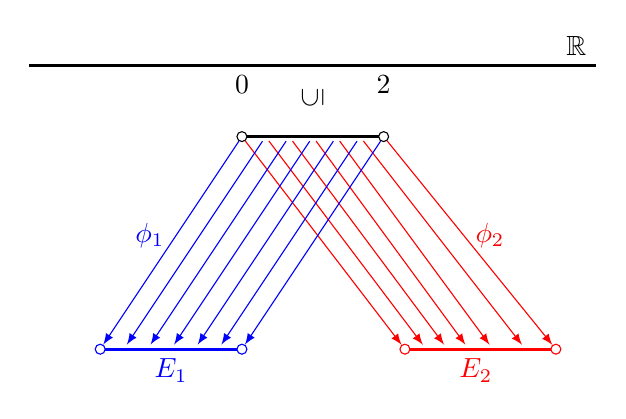
\begin{tikzpicture}[>=latex, scale=0.9]
  \draw[very thick] (0,5)--(8,5);
  \node[above left] at (8,5) {$\mathbb{R}$};
  \draw[very thick] (3,4)--(5,4);
  \draw[fill=white] (3,4) circle(2pt); \draw[fill=white] (5,4) circle(2pt);
  \node[rotate=90] at (4,4.55) {$\subseteq$};
  \node[below] at (3,5) {$0$}; \node[below] at (5,5) {$2$};
  \draw[blue, very thick] (1,1)--(3,1);
  \draw[blue,fill=white] (1,1) circle(2pt); \draw[blue,fill=white] (3,1) circle(2pt);
  \node[blue,below] at (2,1) {$E_1$};
  \draw[red, very thick] (5.3,1)--(7.43,1);
  \draw[red,fill=white] (5.3,1) circle(2pt); \draw[red,fill=white] (7.43,1) circle(2pt);
  \node[red,below] at (6.3,1) {$E_2$};
  \foreach \i/\rx in {0/5.3, 1/5.6, 2/5.9, 3/6.2, 4/6.54, 5/7.0, 6/7.43}{
    \draw[blue,->,shorten >=2pt,shorten <=2pt] ($(3,4)+\i*(0.3333,0)$)--($(1,1)+\i*(0.3333,0)$);
    \draw[red,->,shorten >=2pt,shorten <=2pt] ($(3,4)+\i*(0.3333,0)$)--(\rx,1);
  }
  \node[blue] at (1.7,2.6) {$\phi_1$};
  \node[red] at (6.5,2.6) {$\phi_2$};
\end{tikzpicture}
\end{document}
